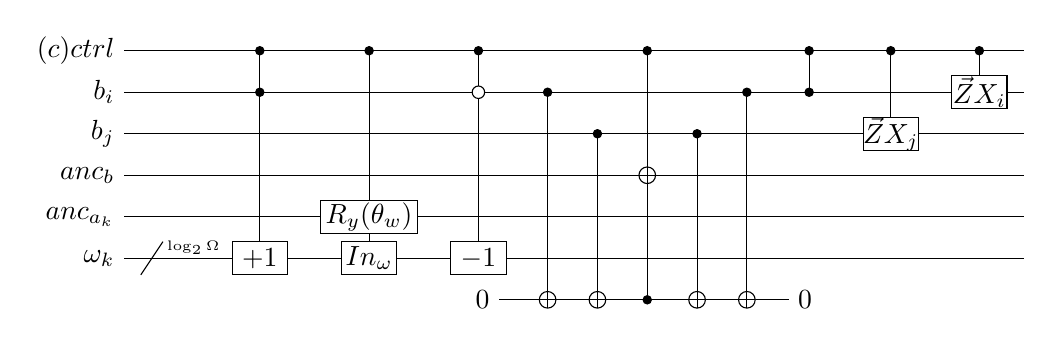
\begin{tikzpicture}[scale=1.000000,x=1pt,y=1pt]
\filldraw[color=white] (0.000000, -7.500000) rectangle (325.000000, 97.500000);
% Drawing wires
% Line 1: ctrl W \text{(c) }ctrl
\draw[color=black] (0.000000,90.000000) -- (325.000000,90.000000);
\draw[color=black] (0.000000,90.000000) node[left] {$\text{(c) }ctrl$};
% Line 2: i W b_i
\draw[color=black] (0.000000,75.000000) -- (325.000000,75.000000);
\draw[color=black] (0.000000,75.000000) node[left] {$b_i$};
% Line 3: j W b_j
\draw[color=black] (0.000000,60.000000) -- (325.000000,60.000000);
\draw[color=black] (0.000000,60.000000) node[left] {$b_j$};
% Line 4: anc_b W anc_b
\draw[color=black] (0.000000,45.000000) -- (325.000000,45.000000);
\draw[color=black] (0.000000,45.000000) node[left] {$anc_b$};
% Line 5: anc_a W anc_{a_k}
\draw[color=black] (0.000000,30.000000) -- (325.000000,30.000000);
\draw[color=black] (0.000000,30.000000) node[left] {$anc_{a_k}$};
% Line 6: k W \omega_k
\draw[color=black] (0.000000,15.000000) -- (325.000000,15.000000);
\draw[color=black] (0.000000,15.000000) node[left] {$\omega_k$};
% Line 7: c0 W 0 0
\draw[color=black] (128.000000,0.000000) -- (247.500000,0.000000);
% Done with wires; drawing gates
% Line 9: k / ^{\log_2{\Omega}}
\draw (6.000000, 9.000000) -- (14.000000, 21.000000);
\draw (12.000000, 18.000000) node[right] {$\scriptstyle{^{\log_2{\Omega}}}$};
% Line 10: ctrl i j anc_b anc_a k c0 LABEL width=1
% Line 12: k G width=20 $+1$ ctrl i
\draw (49.000000,90.000000) -- (49.000000,15.000000);
\begin{scope}
\draw[fill=white] (49.000000, 15.000000) +(-45.000000:14.142136pt and 8.485281pt) -- +(45.000000:14.142136pt and 8.485281pt) -- +(135.000000:14.142136pt and 8.485281pt) -- +(225.000000:14.142136pt and 8.485281pt) -- cycle;
\clip (49.000000, 15.000000) +(-45.000000:14.142136pt and 8.485281pt) -- +(45.000000:14.142136pt and 8.485281pt) -- +(135.000000:14.142136pt and 8.485281pt) -- +(225.000000:14.142136pt and 8.485281pt) -- cycle;
\draw (49.000000, 15.000000) node {$+1$};
\end{scope}
\filldraw (49.000000, 90.000000) circle(1.500000pt);
\filldraw (49.000000, 75.000000) circle(1.500000pt);
% Line 13: anc_a G:width=35 $R_y(\theta_w)$ k G:width=20 $In_\omega$ ctrl
\draw (88.500000,90.000000) -- (88.500000,15.000000);
\begin{scope}
\draw[fill=white] (88.500000, 30.000000) +(-45.000000:24.748737pt and 8.485281pt) -- +(45.000000:24.748737pt and 8.485281pt) -- +(135.000000:24.748737pt and 8.485281pt) -- +(225.000000:24.748737pt and 8.485281pt) -- cycle;
\clip (88.500000, 30.000000) +(-45.000000:24.748737pt and 8.485281pt) -- +(45.000000:24.748737pt and 8.485281pt) -- +(135.000000:24.748737pt and 8.485281pt) -- +(225.000000:24.748737pt and 8.485281pt) -- cycle;
\draw (88.500000, 30.000000) node {$R_y(\theta_w)$};
\end{scope}
\begin{scope}
\draw[fill=white] (88.500000, 15.000000) +(-45.000000:14.142136pt and 8.485281pt) -- +(45.000000:14.142136pt and 8.485281pt) -- +(135.000000:14.142136pt and 8.485281pt) -- +(225.000000:14.142136pt and 8.485281pt) -- cycle;
\clip (88.500000, 15.000000) +(-45.000000:14.142136pt and 8.485281pt) -- +(45.000000:14.142136pt and 8.485281pt) -- +(135.000000:14.142136pt and 8.485281pt) -- +(225.000000:14.142136pt and 8.485281pt) -- cycle;
\draw (88.500000, 15.000000) node {$In_\omega$};
\end{scope}
\filldraw (88.500000, 90.000000) circle(1.500000pt);
% Line 14: k G width=20 $-1$ ctrl -i
\draw (128.000000,90.000000) -- (128.000000,15.000000);
\begin{scope}
\draw[fill=white] (128.000000, 15.000000) +(-45.000000:14.142136pt and 8.485281pt) -- +(45.000000:14.142136pt and 8.485281pt) -- +(135.000000:14.142136pt and 8.485281pt) -- +(225.000000:14.142136pt and 8.485281pt) -- cycle;
\clip (128.000000, 15.000000) +(-45.000000:14.142136pt and 8.485281pt) -- +(45.000000:14.142136pt and 8.485281pt) -- +(135.000000:14.142136pt and 8.485281pt) -- +(225.000000:14.142136pt and 8.485281pt) -- cycle;
\draw (128.000000, 15.000000) node {$-1$};
\end{scope}
\filldraw (128.000000, 90.000000) circle(1.500000pt);
\draw[fill=white] (128.000000, 75.000000) circle(2.250000pt);
% Line 16: c0 START
\draw[color=black] (135.500000,0.000000) node[fill=white,left,minimum height=15.000000pt,minimum width=15.000000pt,inner sep=0pt] {\phantom{$0$}};
\draw[color=black] (135.500000,0.000000) node[left] {$0$};
% Line 17: i +c0
\draw (153.000000,75.000000) -- (153.000000,0.000000);
\filldraw (153.000000, 75.000000) circle(1.500000pt);
\begin{scope}
\draw[fill=white] (153.000000, 0.000000) circle(3.000000pt);
\clip (153.000000, 0.000000) circle(3.000000pt);
\draw (150.000000, 0.000000) -- (156.000000, 0.000000);
\draw (153.000000, -3.000000) -- (153.000000, 3.000000);
\end{scope}
% Line 18: j +c0
\draw (171.000000,60.000000) -- (171.000000,0.000000);
\filldraw (171.000000, 60.000000) circle(1.500000pt);
\begin{scope}
\draw[fill=white] (171.000000, 0.000000) circle(3.000000pt);
\clip (171.000000, 0.000000) circle(3.000000pt);
\draw (168.000000, 0.000000) -- (174.000000, 0.000000);
\draw (171.000000, -3.000000) -- (171.000000, 3.000000);
\end{scope}
% Line 19: ctrl c0 +anc_b
\draw (189.000000,90.000000) -- (189.000000,0.000000);
\filldraw (189.000000, 90.000000) circle(1.500000pt);
\filldraw (189.000000, 0.000000) circle(1.500000pt);
\begin{scope}
\draw[fill=white] (189.000000, 45.000000) circle(3.000000pt);
\clip (189.000000, 45.000000) circle(3.000000pt);
\draw (186.000000, 45.000000) -- (192.000000, 45.000000);
\draw (189.000000, 42.000000) -- (189.000000, 48.000000);
\end{scope}
% Line 20: j +c0
\draw (207.000000,60.000000) -- (207.000000,0.000000);
\filldraw (207.000000, 60.000000) circle(1.500000pt);
\begin{scope}
\draw[fill=white] (207.000000, 0.000000) circle(3.000000pt);
\clip (207.000000, 0.000000) circle(3.000000pt);
\draw (204.000000, 0.000000) -- (210.000000, 0.000000);
\draw (207.000000, -3.000000) -- (207.000000, 3.000000);
\end{scope}
% Line 21: i +c0
\draw (225.000000,75.000000) -- (225.000000,0.000000);
\filldraw (225.000000, 75.000000) circle(1.500000pt);
\begin{scope}
\draw[fill=white] (225.000000, 0.000000) circle(3.000000pt);
\clip (225.000000, 0.000000) circle(3.000000pt);
\draw (222.000000, 0.000000) -- (228.000000, 0.000000);
\draw (225.000000, -3.000000) -- (225.000000, 3.000000);
\end{scope}
% Line 22: c0 END
\draw[color=black] (240.000000,0.000000) node[fill=white,right,minimum height=15.000000pt,minimum width=15.000000pt,inner sep=0pt] {\phantom{$0$}};
\draw[color=black] (240.000000,0.000000) node[right] {$0$};
% Line 24: ctrl i
\draw (247.500000,90.000000) -- (247.500000,75.000000);
\filldraw (247.500000, 90.000000) circle(1.500000pt);
\filldraw (247.500000, 75.000000) circle(1.500000pt);
% Line 26: j G width=20 $\vec{Z}X_j$ ctrl
\draw (277.000000,90.000000) -- (277.000000,60.000000);
\begin{scope}
\draw[fill=white] (277.000000, 60.000000) +(-45.000000:14.142136pt and 8.485281pt) -- +(45.000000:14.142136pt and 8.485281pt) -- +(135.000000:14.142136pt and 8.485281pt) -- +(225.000000:14.142136pt and 8.485281pt) -- cycle;
\clip (277.000000, 60.000000) +(-45.000000:14.142136pt and 8.485281pt) -- +(45.000000:14.142136pt and 8.485281pt) -- +(135.000000:14.142136pt and 8.485281pt) -- +(225.000000:14.142136pt and 8.485281pt) -- cycle;
\draw (277.000000, 60.000000) node {$\vec{Z}X_j$};
\end{scope}
\filldraw (277.000000, 90.000000) circle(1.500000pt);
% Line 27: i G width=20 $\vec{Z}X_i$ ctrl
\draw (309.000000,90.000000) -- (309.000000,75.000000);
\begin{scope}
\draw[fill=white] (309.000000, 75.000000) +(-45.000000:14.142136pt and 8.485281pt) -- +(45.000000:14.142136pt and 8.485281pt) -- +(135.000000:14.142136pt and 8.485281pt) -- +(225.000000:14.142136pt and 8.485281pt) -- cycle;
\clip (309.000000, 75.000000) +(-45.000000:14.142136pt and 8.485281pt) -- +(45.000000:14.142136pt and 8.485281pt) -- +(135.000000:14.142136pt and 8.485281pt) -- +(225.000000:14.142136pt and 8.485281pt) -- cycle;
\draw (309.000000, 75.000000) node {$\vec{Z}X_i$};
\end{scope}
\filldraw (309.000000, 90.000000) circle(1.500000pt);
% Done with gates; drawing ending labels
% Done with ending labels; drawing cut lines and comments
% Done with comments
\end{tikzpicture}
